\documentclass[a4paper,11pt]{article}

\usepackage[spanish]{babel}
\usepackage[utf8]{inputenc}

\usepackage{amsmath}
\usepackage{siunitx}

\usepackage{graphicx}
\usepackage{float}
\usepackage[font=small,labelfont=bf]{caption}

\usepackage{booktabs}
\usepackage{multirow}

\usepackage{hyperref}
\hypersetup{
    bookmarks=true,         % show bookmarks bar?
    unicode=false,          % non-Latin characters in Acrobat’s bookmarks
    pdftoolbar=true,        % show Acrobat’s toolbar?
    pdfmenubar=true,        % show Acrobat’s menu?
    pdffitwindow=false,     % window fit to page when opened
    pdfstartview={FitH},    % fits the width of the page to the window
    pdftitle={My title},    % title
    pdfauthor={Author},     % author
    pdfsubject={Subject},   % subject of the document
    pdfcreator={Creator},   % creator of the document
    pdfproducer={Producer}, % producer of the document
    pdfkeywords={keyword1, key2, key3}, % list of keywords
    pdfnewwindow=true,      % links in new PDF window
    colorlinks=true,       % false: boxed links; true: colored links
    linkcolor=blue,          % color of internal links (change box color with linkbordercolor)
    citecolor=green,        % color of links to bibliography
    filecolor=magenta,      % color of file links
    urlcolor=cyan           % color of external links
}

\title{Estabilización de temperatura mediante lazos de control}
\date{\today}
\author{Micaela Toscani, Axel Lacapmesure y Guillermo Brinatti}

\begin{document}
\maketitle



\section{Introducción}

El objetivo del presente trabajo consiste en implementar un sistema de control de temperaturas en un prototipo de planta utilizando un lazo de control. Para ello empleamos un sensor de temperatura electrónico a modo de sensor en el lazo y una celda Peltier sobre la cual se variará su corriente a modo de actuador. Estos elementos fueron controlados mediante una placa de adquisición y una aplicación programada en lenguaje Python, la cual implementa la lógica del lazo de control y la comunicación con los dispositivos. En la sección \ref{sec:software} detallamos la aplicación mediante la cual realizamos la comunicación con los dispositivos, en la sección \ref{sec:daq} caracterizamos el funcionamiento de la placa de adquisición y, por último, en la sección \ref{sec:control_temperatura} describimos y evaluamos el desempeño de los distintos esquemas de lazos de control realizados.

\section{Desarrollo de la aplicación de adquisición}
\label{sec:software}

Para implementar el lazo de control se utilizó una placa de adquisición \emph{National Instruments} NI-USB6210, adquiriendo la señal del sensor mediante un canal de entrada analógico de la placa de adquisición, y controlando el actuador mediante una salida de contador digital en modo PWM, que permitía generar trenes de pulsos con frecuencia de repetición y anchos configurables.	El control de la placa de adquisición fue llevado a cabo a partir de programar una biblioteca propia en lenguaje Python \cite{repo}. La misma incluyó funciones orientadas al usuario final destinadas a utilizar el dispositivo para la adquisición de datos y la generación de trenes de pulsos configurables, tanto en los modos de disparo único como de ejecución continua. Para ello empleamos la biblioteca \emph{\href{https://nidaqmx-python.readthedocs.io}{nidaqmx}} propia del fabricante de la placa de adquisición \cite{nidaqmx}, y que provee una API para la configuración del dispositivo y para su comunicación a través de los controladores del mismo.
	
	Las funciones de usuario final se encargaron de la configuración de los canales de entrada analógicos y salidas de contadores, de la adquisición de una muestra finita de largo arbitrario, y de la adquisición continua de datos en simultáneo con la generación de pulsos de anchos variables. En la figura \ref{fig:flujo_software} se muestra un diagrama de flujo de una ejecución típica para la adquisición y generación de pulsos en modo continuo. Asimismo la biblioteca incluyó los elementos necesarios para la implementación del lazo de control que se discutirá en la sección \ref{sec:control_temperatura}, a saber, las estructuras que manejan la entrada de datos de sensado, que calculan la señal de error y que generan la señal de hacia el actuador.
	
	\begin{figure}[h!]
        \centering
        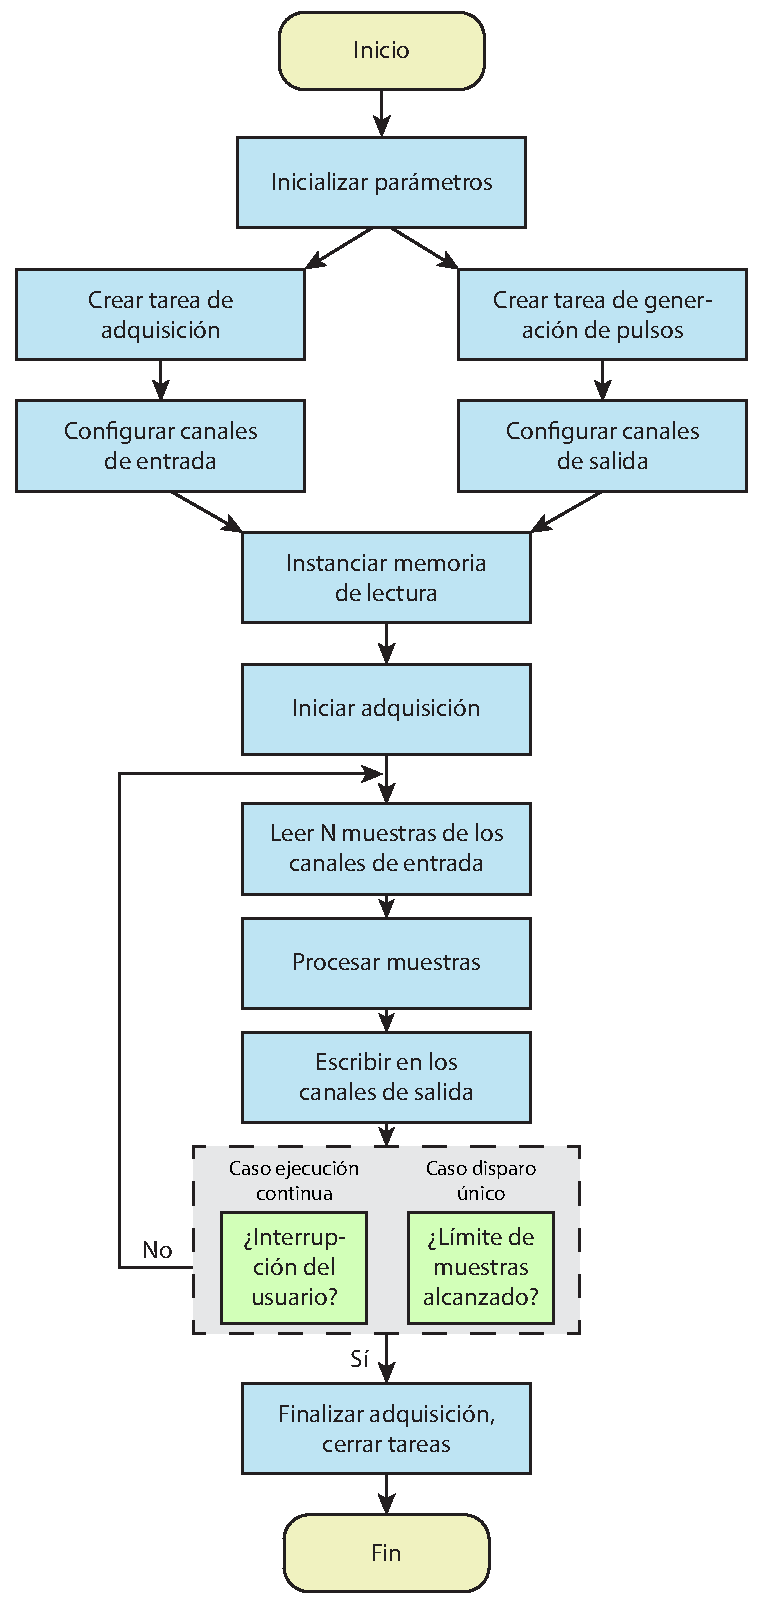
\includegraphics[height=.9\textheight]{figs/flujo_software.pdf}
        \caption{Diagrama de flujo para la aplicación de adquisición y generación de pulsos en modo de disparo único y ejecución continua.}
        \label{fig:flujo_software}
    \end{figure}	
	
	El la adquisición de lectura y escritura se basa en un bucle que en cada iteración adquiere una ventana de datos con un número fijo de muestras, las procesa y por último escribe la configuración de los pulsos de salida, esto es, su frecuencia de repetición y su ancho. Para el funcionamiento de este esquema se asume que el tiempo de ejecución de las instrucciones dentro de cada iteración es menor al tiempo que demora la adquisición de las muestras, de manera que no se produzcan sobrecargas en el \emph{buffer} de la placa de adquisición. Bajo el modo de disparo único, las sucesivas ventanas temporales se concatenan en una variable de salida preinicializada, y el bucle finaliza cuando el número de muestras adquiridas alcanza el número total configurado. Bajo el modo de ejecucuón continua, las ventanas temporales se sobreescriben, y el bucle finaliza cuando el usuario interrumpe manualmente la ejecución del programa con el comando de teclado. En ambos casos, la finalización del bucle desencadena la etapa de cierre de comunicaciones y, eventualmente, el gráfico y guardado de los datos.
	
	El la adquisición de lectura y escritura se basa en un bucle que en cada iteración adquiere una ventana de datos con un número fijo de muestras, las procesa y por último escribe la configuración de los pulsos de salida, esto es, su frecuencia de repetición y su ancho. Para el funcionamiento de este esquema se asume que el tiempo de ejecución de las instrucciones dentro de cada iteración es menor al tiempo que demora la adquisición de las muestras, de manera que no se produzcan sobrecargas en el \emph{buffer} de la placa de adquisición. Bajo el modo de disparo único, las sucesivas ventanas temporales se concatenan en una variable de salida preinicializada, y el bucle finaliza cuando el número de muestras adquiridas alcanza el número total configurado. Bajo el modo de ejecucuón continua, las ventanas temporales se sobreescriben, y el bucle finaliza cuando el usuario interrumpe manualmente la ejecución del programa con el comando de teclado. En ambos casos, la finalización del bucle desencadena la etapa de cierre de comunicaciones y, eventualmente, el gráfico y guardado de los datos.	

\section{Caracterización de la placa de adquisición}
\label{sec:daq}

Se realizó una caracterización de la placa de adquisición en la que se propuso investigar los efectos de \textit{aliasing}, los tiempos asociados al multiplexado y el efecto del \textit{settling time} de la placa en las mediciones analógicas. 

En primer lugar, para observar el efecto que produce submuestrear una señal, se alimento una entrada analógica de la placa DAQ con una señal sinusoidal de frecuencia controlada producida por un generador de funciones. Se fijó la frecuencia de muestreo de la placa en $f_s$ = 10 kHz y se barrió la frecuencia de la señal de entrada $f_r$ entre valores mucho menores y mucho mayores a dicha frecuencia. El tiempo de integración se eligió grande, de manera de minimizar la introducción de frecuencias espúreas en la señal dadas por el tamaño de la ventana temporal. Luego, usando un algoritmo de tranformada rápida de Fourier (FFT), se obtuvo para cada frecuencia de entrada su frecuencia medida $f_m$, a partir del valor máximo del módulo de la FFT. En la figura \ref{fig:aliasing} se muestran los resultados de este experimento. Para frecuencias menores a la frecuencia de Nyquist ($f_r/f_s = 0.5$) se observa como la frecuencia medida se corresponde con la de la señal de entrada. A partir de este punto, se puede ver como el algoritmo devuelve de manera consistente valores menores a la frecuencia de Nyquist mostrando el fenómeno de aliasing. En particular, el punto donde $f_r = f_s$ devuelve un valor de frecuencia nulo, que se corresponde con estar muestreando la señal en el mismo punto del período cada vez.

\begin{figure}[!ht]
\centering
\includegraphics[width=\textwidth]{figs/alliasing.png}
\caption{Frecuencia medida en función de la frecuencia real comparadas con la tasa de muestreo.}
\label{fig:aliasing}
\end{figure}

Para entender la forma en que la placa multiplexa las señales, se diseño un experimento en el que se busca medir cual es la relación entre los tiempos en los que se efectúa la adquisición para cada canal analógico. Para hacer esto se utilizó un generador de funciones para producir una rampa de tensión de igual frecuencia a la adquisición de la placa. La misma señal se alimentó varios canales analógicos de la placa. Bajo esta disposición, el valor de tensión medido para cada canal codifica el instante en el que se produjo dicha medición, ya que la señal de entrada se encuentra variando de manera rápida y controlada dentro del tiempo en que la placa está realizando el multiplexado de las señales. 

\begin{figure}[!ht]
\centering
\includegraphics[width=\textwidth]{figs/multiplex.png}
\caption{Caracterización del multiplexor midiendo una rampa de tensión de manera simultanea en tres canales analógicos.}
\label{fig:multiplex}
\end{figure}


Un resultado típico de este experimento donde se utilizaron tres canales analógicos y una frecuencia de muestreo de 40 kHz se muestra en la figura \ref{fig:multiplex}. En la misma se observan dos eventos de medición separados un período de muestreo. Para cada uno se puede ver que la diferencia entre los valores de tensión registrados en cada canal es la misma y el orden se repite en cada adquisición. A partir de conocer los parámetros de la rampa de tensión utilizada se puede calcular que la diferencia de tensión observada corresponde exactamente a un tercio del período de muestreo. El mismo resultado se obtiene si se utilizan cuatro canales, donde ahora las mediciones se distribuirán equiespaciadamente entre cuatro el período de muestreo. El mismo resultado se observa al cambiar la frecuencia de muestreo. Esto demuestra que la placa de adquisición va digitalizando los canales analógicos de manera secuencial y a intervalos constantes y equiespaciados temporalmente dentro del período de muestreo.

Para finalizar la caracterización de la placa se midió la influencia del \textit{settling time} en las mediciones. Para hacer esto se configuraron dos canales analógicos consecutivos de la placa en las escalas de medición extremas (-200 mV a 200 mV y -10 V a 10 V). Luego se conectó el primero a tierra y el segundo a la referencia de 5 V de la misma placa. A continuación se realizó un barrido de frecuencias de adquisición registrando la tensión detectada en cada canal. El resultado de este experimento se muestra en las figuras \ref{fig:settling1} y \ref{fig:settling2}, donde se graficó la diferencia de tensión medida respecto de la esperada para cada canal. Se observa para los dos casos que a medida que la frecuencia aumenta (y luego se cambia cada vez más rápido de un canal a otro) se obtiene una pequeña señal residual en la dirección de la señal del canal vecino (positiva para el conectado a tierra y negativa para el de 5 V). Esto muestra que la señal está afectada, a frecuencias altas, por el tiempo que tarda la placa en preparar el acondicionamiento de la señal previo a su digitalización.  

\begin{figure}[h!]
\centering
\includegraphics[height=.42\textheight]{figs/settling0V.png}
\caption{Señal medida en una entrada conectada a tierra, configurada en $\pm$200 mV contigua a otra configurada en $\pm$10 V en función de la frecuencia de muestreo.}
\label{fig:settling1}
\end{figure}

\begin{figure}[h!]
\centering
\includegraphics[height=.42\textheight]{figs/settling5V.png}
\caption{Variación de la tensión medida en una entrada conectada a 5 V, configurada en $\pm$10 V contigua a otra configurada en $\pm$200 mV en función de la frecuencia de muestreo.}
\label{fig:settling2}
\end{figure}

\clearpage
\section{Control de temperatura}
\label{sec:control_temperatura}

Se construyó una planta con actuadores y sensores de temperatura con el
objetivo de ser utilizada para implementar distintos lazos de control,
en la figura \ref{fig:planta} se muestra un diagrama en bloques de la
misma.  Se utilizó como actuador una celda \emph{peltier} modelo
TEC1-12706 controlada mediante una señal PWM cuyo ciclo de trabajo podía
ser modificado por la placa de adquisición utilizada. Se utilizó como
sensor de temperatura el integrado LM35, su señal de salida es lineal y
cada grado Celcius equivale a \SI{10}{\mV}. 

\begin{figure}[!ht]
\centering
\includegraphics[width=0.8\textwidth]{figs/Planta}
\caption{Diagrama en bloques de la planta implementada.}
\label{fig:planta}
\end{figure}

\subsection{Implementación de un lazo de control}
Con el objetivo de mantener constante la
señal de temperatura medida en un valor de refencia establecido se
implentó un lazo de control con la siguiente lógica,
\begin{equation*}
\text{duty cycle (t+1)} = \text{duty cycle (t)} + a * (\text{temp SET}
- \text{temp (t)})
\end{equation*}

En las figuras \ref{fig:lazo_duty} y \ref{fig:lazo_temp} se muestra la
evolución temporal de las señales de ciclo de trabajo del actuador y de
tempratura medida para cuatro valores distintos de la constante de
proporcionalidad \emph{a}.

\begin{figure}[!h]
\centering
\includegraphics[width=\textwidth]{figs/lazo_duty}
\caption{Evolución temporal de la señal de ciclo de trabajo del actuador
de temperatura para distintos valores de la constante de
proporcionalidad \emph{a}.}
\label{fig:lazo_duty}
\end{figure}

\begin{figure}[!h]
\centering
\includegraphics[width=\textwidth]{figs/lazo_temp}
\caption{Evolución temporal de la señal de temperatura para distintos
valores de la constante de proporcionalidad \emph{a}.}
\label{fig:lazo_temp}
\end{figure}

\clearpage
\subsection{Implementación de un lazo de control PID}

Se implementó un controloador del tipo PID para mantener estable la
señal de temperatura de la planta utilizada. En la figura
\ref{fig:PID_diagrama} se muestra un diagrama en bloques del control
implementado. Para encontrar los parámetros que optimizan el
funcionamiento del control PID se utilizó el método de ajuste
\emph{Cohen-Coon}. El mismo consiste en excitar la planta con una señal
escalón y medir de la respuesta de la misma ciertos parámetros
característicos como se muestra en la figura
\ref{fig:CohenCoon_StepTest}. Una vez obtenidos los parámetros
necesarios, las distintas constantes de proporcionalidad de cada término
del control PID se ajustan siguiendo las reglas que se muestran en la
figura \ref{fig:CohenCoon_Rules}. Por último, alrededor de los valores devueltos por el ajuste de \emph{Cohen-Coon} se ajustan manualmente las ganancias buscando atenuar sobrepicos, errores estacionarios, tiempos de respuesta y estabilidad.

\begin{figure}[H]
\centering
\includegraphics[width=0.8\textwidth]{figs/PID_diagrama}
\caption{Diagrama en bloques de un controlador PID en un lazo realimentado.}
\label{fig:PID_diagrama}
\end{figure}

\begin{figure}[H]
\centering
\includegraphics[width=0.8\textwidth]{figs/CohenCoon_StepTest}
\caption{Ejemplo de la prueba de escalón para el ajuste de parámetros PID mediante el
método \emph{Cohen-Coon}}
\label{fig:CohenCoon_StepTest}
\end{figure}

\begin{figure}[!ht]
\centering
\includegraphics[width=\textwidth]{figs/CohenCoon_Rules}
\caption{Reglas de ajuste del método \emph{Cohen-Coon} para los
\label{fig:CohenCoon_Rules}
distintos tipos de controladores.}
\end{figure}

Se implementó el controlador PID en tres etapas: primero solo se utilizó
un control proporcional (P), luego se agregó un término integral al
mismo (PI), el cual permitió reducir el error estacionario del controlador
proporcional, y finalmente se agregó un término derivativo (PID) con el
objetivo de disminuir el sobrepico inicial en la señal de temperatura. Para implementar el término diferencial se computó la derivada numérica entre dos adquisiciones consecutivas de la señal sensada, mientras que para implementar el término integral $I$ se utilizó la relación
\begin{equation}
	I_{k+1} = \alpha I_k + K_i e_k
\end{equation}
donde $I_k$ y $e_k$ son respectivamente el término integral y la señal de error en el paso $k$, $K_i$ es la ganancia del término integral y $\alpha<1$ es una constante que regula el tiempo de integración, y que fue tomada igual a \SI{0.25}{} en todo nuestro trabajo. Los resultados obtenidos para los tres lazos mencionados se muestran en las figuras \ref{fig:P_temp}, \ref{fig:PI_temp} y \ref{fig:PID_temp}.

\begin{figure}[!h]
\centering
\includegraphics[width=0.8\textwidth]{figs/P_temp}
\caption{Evolución temporal de la señal de temperatura utilizando
un controlador de tipo proporcional (P), registrada para tres valores
disintos de la constante de proporcionalidad.}
\label{fig:P_temp}
\end{figure}

\begin{figure}[!h]
\centering
\includegraphics[width=0.8\textwidth]{figs/PI_temp}
\caption{Evolución temporal de la señal de temperatura cuando se agrega
un término integral al controlador (PI).}
\label{fig:PI_temp}
\end{figure}

\begin{figure}[!h]
\centering
\includegraphics[width=0.8\textwidth]{figs/PID_temp}
\caption{Evolución temporal de la señal de temperatura cuando se agrega
un término derivativo al controlador (PID).}
\label{fig:PID_temp}
\end{figure}

En el caso del lazo proporcional, para todas los valores de ganancia estudiados se obtuvieron tiempos de estabilización similares, del orden de \SI{100}{\s}. Una vez estabilizado, la temperatura presentó fluctuaciones menores a \SI{\pm 2.5}{\percent} debido al ruido de la planta, el cual también afectó a la señal del ciclo de trabajo. Estas fluctuaciones no pudieron ser atenuadas, de modo que estuvieron presentes en todas los lazos configurados en nuestro trabajo. Asimismo para todos los valores de ganancia del lazo proporcional se observó un error estacionario, con valores entre \SI{0.2}{\celsius} y \SI{1}{\celsius}, y que mejoró para mayores valores de la ganancia del lazo. Al introducir un término integral se pudo eliminar este error estacionario, introduciendo sobrepicos y alargando el tiempo de estabilización. Finalmente, al introducir el término derivador no se logró eliminar el sobrepico inicial pero en cambio sí se mejoró el tiempo de estabilización, tal como puede verse en la figura \ref{fig:PID_temp}, en especial si consideramos que la temperatura inicial fue menor que para la medición graficada en la figura \ref{fig:PI_temp}.

Por último nos propusimos estudiar la respuesta del sistema ante una perturbación. Para ello cambiamos la configuración de la planta inicial por aquella esquematizada en la figura \ref{fig:planta2}, en donde pasamos a medir la temperatura directamente sobre la cara caliente de la celda Peltier, prescindiendo del bloque de aluminio. Una vez que el lazo de control llegó al equilibrio, la perturbación consistió en poner en contacto el bloque de aluminio con dicha cara de la celda Peltier.

\begin{figure}[h!]
\centering
\includegraphics[width=0.8\textwidth]{figs/Planta2}
\caption{Diagrama en bloques de la planta implementada para introducir perturbaciones. Inicialmente prescindimos del bloque de aluminio, el cual fue agregado una vez comenzada la medición a modo de perturbación del sistema.}
\label{fig:planta2}
\end{figure}

Para este caso configuramos las ganancias del lazo PID igual a los valores finales obtenidos para la planta anterior. Bajo esa condición tomamos la medición que graficamos en la figura \ref{fig:PID_temp_peltier}, estableciendo una temperatura de referencia de \SI{50}{\celsius}. Una vez se alcanzó el equilibrio se puso en contacto el bloque de aluminio con la cara de la Peltier, a un tiempo de aproximadamente \SI{250}{\s}. La perturbación introdujo una disminución en la temperatura medida de \SI{0.2}{\celsius}. La señal del ancho de pulso se alteró en consecuencia y no se observa que alcance un nuevo valor estable en la totalidad de la medición. Contrariamente sí observamos que el lazo logra estabilizar temperatura en su valor de referencia en un intervalo de aproximadamente \SI{200}{\s}.

\begin{figure}[H]
\centering
\includegraphics[width=\textwidth]{figs/PID_sobre_peltier.png}
\caption{Evolución temporal de la señal de temperatura (superior) y del ciclo de trabajo (inferior) sensando la temperatura en la cara caliente de la celda Peltier. La perturbación se introduce aproximadamente a los \SI{250}{\s}. El recuadro muestra una ampliación de la temperatura alrededor de la perturbación.}
\label{fig:PID_temp_peltier}
\end{figure}


\begin{thebibliography}{99}

	\bibitem{repo} Repositorio en GitHub de la biblioteca propia utilizada en el trabajo, \href{https://github.com/fotonicaOrg/daq}{URL: https://github.com/fotonicaOrg/daq}, actualizado el 7/11/2018. La biblioteca está programada en el archivo \emph{daq.py}.
	\bibitem{nidaqmx} Documentación de la biblioteca nidaqmx, \href{https://nidaqmx-python.readthedocs.io}{URL: https://nidaqmx-python.readthedocs.io}, accedido el 7/11/2018.


\end{thebibliography}



\end{document}
